\begin{pastexam}[label={px:nccu-108-dsa-03}]{政大資科所 108 學年度 第 3 題}
（問答）

(15\%) A vertex cover of a graph $G=(V,E)$ is a subset of vertices $S\subseteq V$ that includes at
least one endpoint of every edge in $E$. Use dynamic programming to design a linear time algorithm
that outputs the smallest vertex cover in a tree. For example, in the following tree,
$\{\mathrm{A,C,D,F}\}$ is a vertex cover, and $\{\mathrm{C,E,F}\}$ is not a vertex cover. The
smallest vertex cover in the following tree is $\{\mathrm{B,E,G}\}$.
\begin{center}
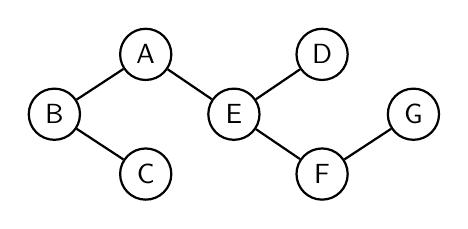
\begin{tikzpicture}[x=0.8cm,y=0.8cm,thick,v/.style={circle,draw,minimum size=6.5mm,inner sep=0pt,font=\sffamily}]
\node[v] (A) at (3.6,-0.6) {A}; \node[v] (B) at (2.15,-1.55) {B}; \node[v] (C) at (3.6,-2.5) {C};
\node[v] (E) at (5.0,-1.55) {E}; \node[v] (D) at (6.4,-0.6) {D}; \node[v] (F) at (6.4,-2.5) {F};
\node[v] (G) at (7.85,-1.55) {G};
\draw (A)--(B) (B)--(C) (A)--(E) (E)--(D) (E)--(F) (F)--(G);
\end{tikzpicture}
\end{center}
\end{pastexam}

\begin{pastsoln}
\textbf{子問題}。 任選一點 $r$ 當根（資結書第~18.8.1~節）。 對每個點 $v$ 記兩個值：$\mathit{take}[v]$ 是
子樹 $T_v$ 的頂點覆蓋中\textbf{包含} $v$ 的最小大小（只看 $T_v$ 裡的邊），$\mathit{skip}[v]$ 是\textbf{不含}
$v$ 的最小大小。

\textbf{遞迴式}。 $v$ 在覆蓋裡時，邊 $\{v, u\}$ 都已經蓋住，每個子節點 $u$ 選不選都可以，取小的；$v$ 不在
覆蓋裡時，邊 $\{v, u\}$ 只能靠 $u$ 蓋住，每個子節點都必須選：
\[
\mathit{take}[v] = 1 + \sum_{u} \min\bigl(\mathit{take}[u], \mathit{skip}[u]\bigr), \qquad
\mathit{skip}[v] = \sum_{u} \mathit{take}[u],
\]
$u$ 跑過 $v$ 的所有子節點；葉節點 $\mathit{take} = 1$、$\mathit{skip} = 0$。 答案是
$\min(\mathit{take}[r], \mathit{skip}[r])$。

\textbf{正確性}。 $T_v$ 的任何覆蓋，限制在 $T_u$ 上仍然蓋住 $T_u$ 的所有邊，所以每個子樹那一部分的大小
至少是該子樹在相應條件下的最小值。 $v$ 選不選定了以後，各子樹之間只透過邊 $\{v, u\}$ 互相影響，這個條件
上面已經寫進去（$v$ 不選時 $u$ 必須選），其餘部分各子樹各自取最小，合起來就是最小（剪下貼上，和資結書
第~18.8.2~節的獨立集相同）。 對子樹大小歸納即得兩個遞迴式正確。

\begin{pseudo}{樹的最小頂點覆蓋}
\Procedure{Tree-VC}{$v, p$}
    \State $\mathit{take}[v] \gets 1$
    \State $\mathit{skip}[v] \gets 0$
    \For{每個 $u \in \mathit{Adj}[v]$}
        \If{$u \ne p$}
            \State \Call{Tree-VC}{$u, v$}
            \State $\mathit{take}[v] \gets \mathit{take}[v] + \min(\mathit{take}[u], \mathit{skip}[u])$
            \State $\mathit{skip}[v] \gets \mathit{skip}[v] + \mathit{take}[u]$
        \EndIf
    \EndFor
\EndProcedure
\Statex
\Procedure{Tree-VC-Pick}{$v, p, \mathit{must}$} \Comment{$\mathit{must}$：父節點沒選，$v$ 一定要選}
    \If{$\mathit{must}$ \OR $\mathit{take}[v] < \mathit{skip}[v]$}
        \State 印出 $v$
        \State $\mathit{must} \gets \FALSE$
    \Else
        \State $\mathit{must} \gets \TRUE$ \Comment{$v$ 沒選，子節點都要選}
    \EndIf
    \For{每個 $u \in \mathit{Adj}[v]$}
        \If{$u \ne p$}
            \State \Call{Tree-VC-Pick}{$u, v, \mathit{must}$}
        \EndIf
    \EndFor
\EndProcedure
\end{pseudo}

先呼叫 $\proc{Tree-VC}(r, \NIL)$，再呼叫 $\proc{Tree-VC-Pick}(r, \NIL, \FALSE)$ 輸出覆蓋；平手時不選。
$\proc{Tree-VC-Pick}$ 在 $v$ 沒被強迫時選 $\mathit{take}$ 和 $\mathit{skip}$ 裡較小的那個，選了 $v$ 就讓
子節點自由，沒選 $v$ 就強迫子節點都選，正好照著遞迴式的取法還原，所以印出的集合大小就是
$\min(\mathit{take}[r], \mathit{skip}[r])$。

\textbf{時間}。 每個點各被兩個程序處理一次，每條邊在兩端各看一次，共 $\Theta(n)$，是線性時間。 $n$ 很大時
把遞迴改成資結書第~18.8.1~節的倒序走訪，避免遞迴太深。

\textbf{題目的樹}。 以 A 為根，A 的子節點是 B、E，B 的是 C，E 的是 D、F，F 的是 G。 後序是 C、B、D、G、F、
E、A：
\begin{center}
\small
\begin{tabular}{ccll}
\toprule
$v$ & 子節點 & $\mathit{take}[v]$ & $\mathit{skip}[v]$ \\
\midrule
C、D、G & -- & $1$ & $0$ \\
B & C & $1 + \min(1, 0) = 1$ & $1$ \\
F & G & $1 + \min(1, 0) = 1$ & $1$ \\
E & D、F & $1 + \min(1, 0) + \min(1, 1) = 2$ & $1 + 1 = 2$ \\
A & B、E & $1 + \min(1, 1) + \min(2, 2) = 4$ & $1 + 2 = 3$ \\
\bottomrule
\end{tabular}
\end{center}
最小頂點覆蓋的大小是 $\min(4, 3) = 3$。 還原：A 的 $\mathit{skip} = 3 < 4$，不選，B、E 一定要選；B 選了，
C 的 $1 > 0$，不選；E 選了，D 不選，F 的 $1 = 1$ 平手，不選，於是 G 一定要選。 輸出 $\{\mathrm{B, E, G}\}$，
和題目給的答案相同。 平手時改成選 F，會得到 $\{\mathrm{B, E, F}\}$，也是大小 $3$ 的頂點覆蓋；大小 $3$ 的
頂點覆蓋只有這兩個。

另一種寫法：先用資結書第~18.8.2~節的最大獨立集 DP（每點權重 $1$），再取補集。 $S$ 是頂點覆蓋若且唯若
$V - S$ 是獨立集：每條邊至少一端在 $S$，等於沒有一條邊兩端都在 $V - S$。 所以最小頂點覆蓋的大小是
$n$ 減去最大獨立集的大小。 這棵樹的最大獨立集 $\{\mathrm{A, C, D, G}\}$ 大小 $4 = 7 - 3$，補集
$\{\mathrm{B, E, F}\}$ 也是最小頂點覆蓋。
\end{pastsoln}
